\chapter{Developed Tools}

This chapter contains an overview of why supplementary tools were deemed necessary for an already working reduction process (\S~\ref{sec:polsalt_limits}), which aspects of the reduction process have been altered, replaced, or added (\S~\ref{sec:mod_tools}, \ref{sec:add_tools}), and finally what an updated reduction process consists of using a combination of all software (\S~\ref{sec:red_proc}).


\section{Limitations of POLSALT and the Need for a Supplementary Tool} \label{sec:polsalt_limits} % Rename

% Why
The creation of supplementary tools for \polsalt spectropolarimetric reductions stem from, primarily, the limitations of the wavelength calibration process and a need for a way to compare wavelength solutions across matching $O$ and $E$ polarization beams. Due to the time-consuming process of recalibrating the wavelength solutions it is not feasible to perform the wavelength calibrations time and time again for any amount of reductions larger than a handful of observations.
\prgph

% PG0300 reasoning
The prime motivation of finding an alternate method of wavelength calibrating the data stemmed from a large backlog of unused data taken using the $PG0300$. The only arc available for the $PG0300$ with a close enough articulation and grating angle ($\sim 10.68$ and $\sim 5.38$, respectively) was the Argon lamp which displayed sparse spectral features with large gaps over the wavelength range at these grating and articulation angles. This often lead to inconsistent wavelength solutions or failed altogether through \polsalt, since minor deviations of identified spectral features may result in large deviations in regions with no spectral features.
\prgph

% How
The chosen solution was to use a well established tool to perform the wavelength calibration - one which allows for rapid recalibrations as well as provides a familiar interface with which the user can analyze their wavelength solutions. \iraf provides this familiar environment and reliability, even considering it's age and \hyperlink{https://github.com/iraf-community/iraf}{limited community development}. Unfortunately, \iraf is unable to parse the file structure implemented by \polsalt as is and formatting of the data structures are necessary for integration purposes. This restructuring works both ways as once the \iraf reductions are complete the format must be reformatted to match that of the \polsalt output such that the reduction process may carry on in \polsalt.
\prgph

\begin{figure}[t]
    \centering
    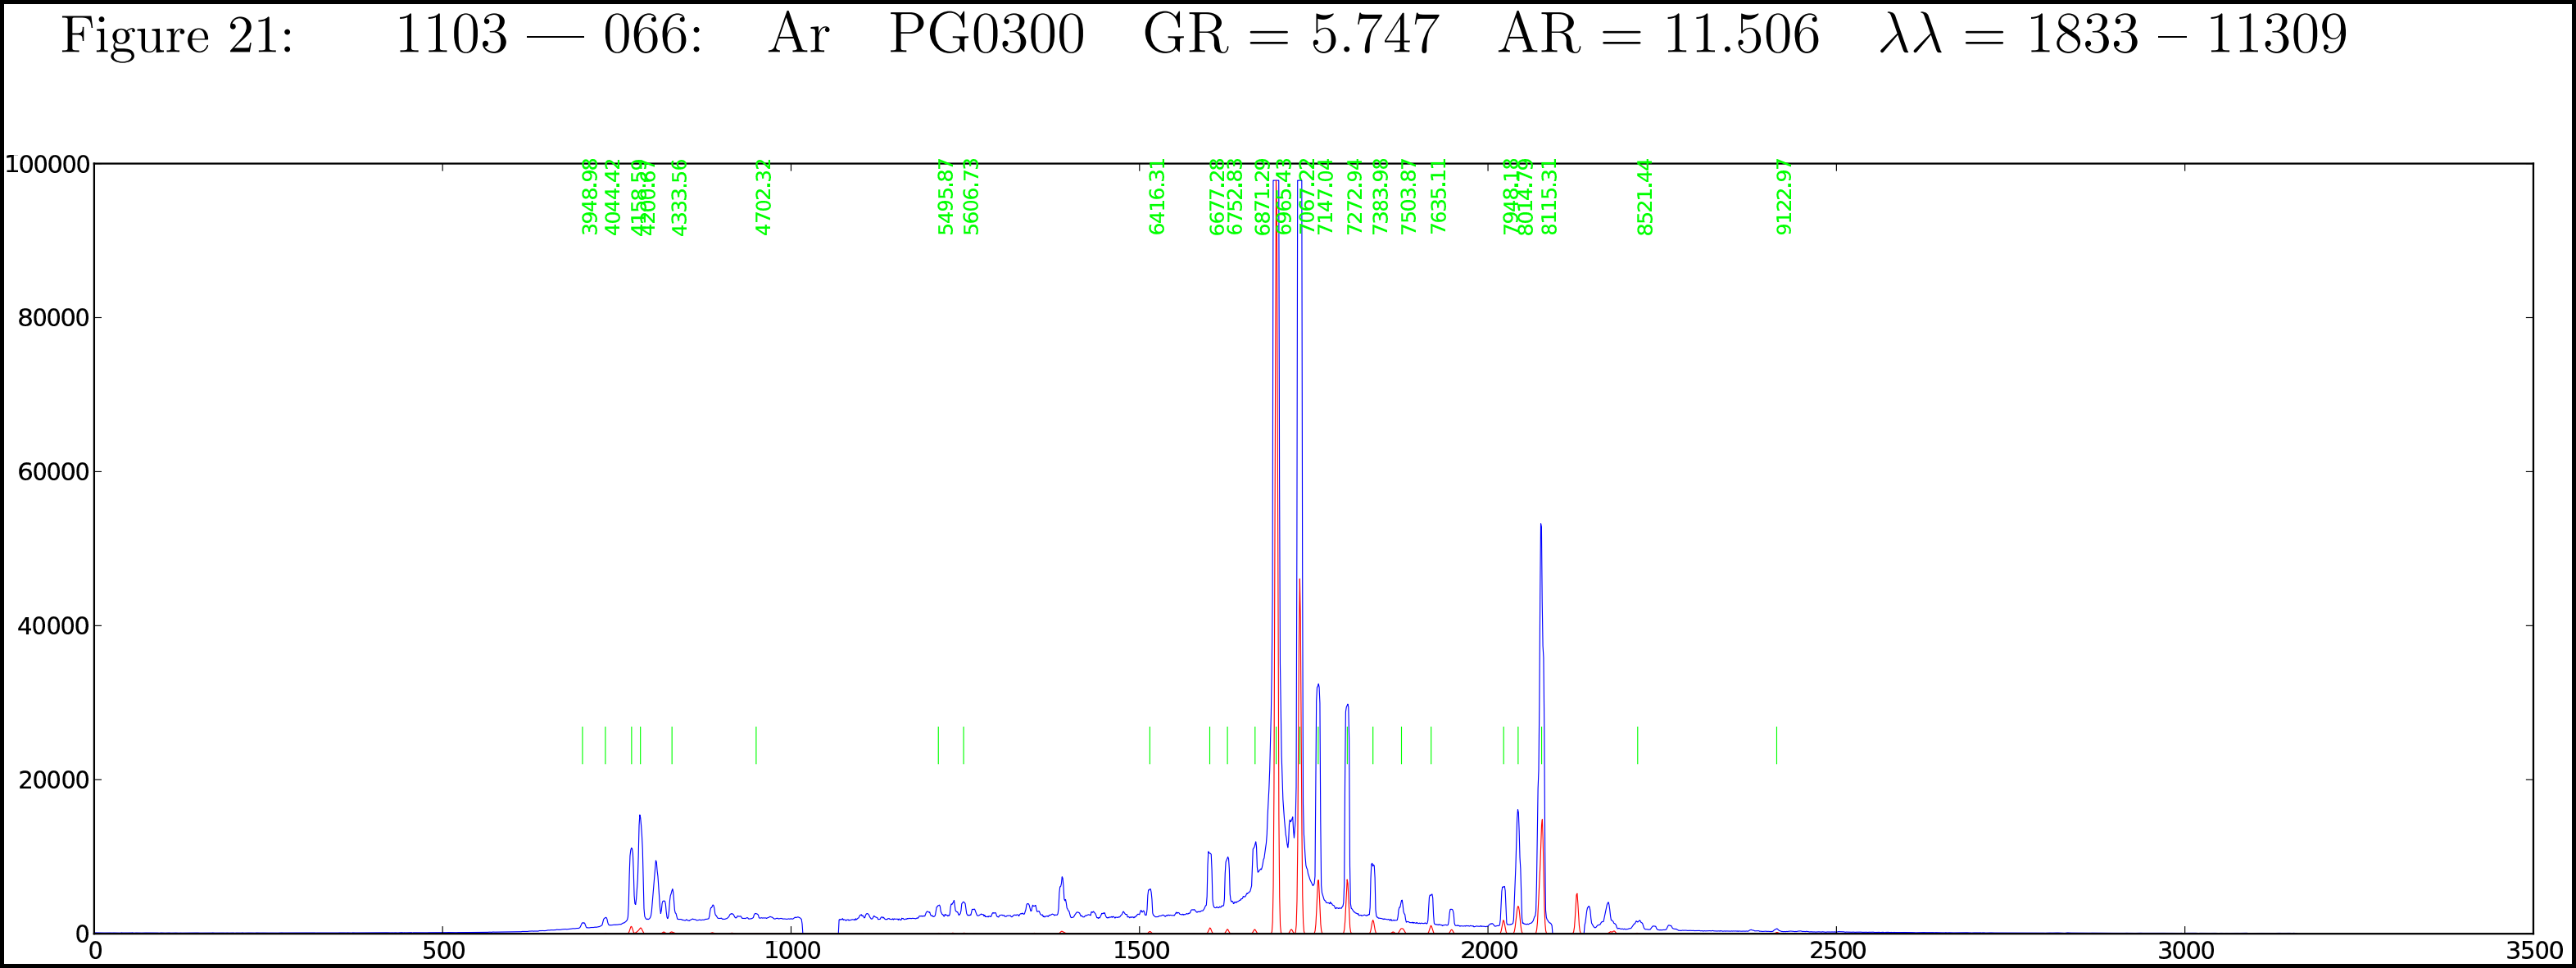
\includegraphics[width = 0.98\textwidth]{figures/3_arc_spectrum.png}
    \caption{One of many Argon arc lamp spectra as provided by \gls{SALT} for line identification. Plot adapted from \gls{SALT}'s published Longslit Line Atlases (as of 2024)\protect\footnotemark}
    \label{fig:ar_arc_salt}
\end{figure}
\footnotetext{\protect\href{https://pysalt.salt.ac.za/lineatlas/plot_line_argon_lores.pdf}{low resolution Ar plot} sourced from \protect\url{https://astronomers.salt.ac.za/data/salt-longslit-line-atlas/}}


\section{Wavelength calibrations - Supplementary Tools and IRAF} \label{sec:mod_tools}

The supplementary tools offer an alternate procedure for wavelength calibrations for the \polsalt pipeline. This procedure can be broken into three unique steps: the parsing of \polsalt data into an \iraf friendly format, from here on referred to as splitting; the wavelength calibration performed in \iraf; and the reformatting of the data with its wavelength calibration back into the format expected by \polsalt, from here on referred to as joining.

\begin{figure}[t]
    \centering
    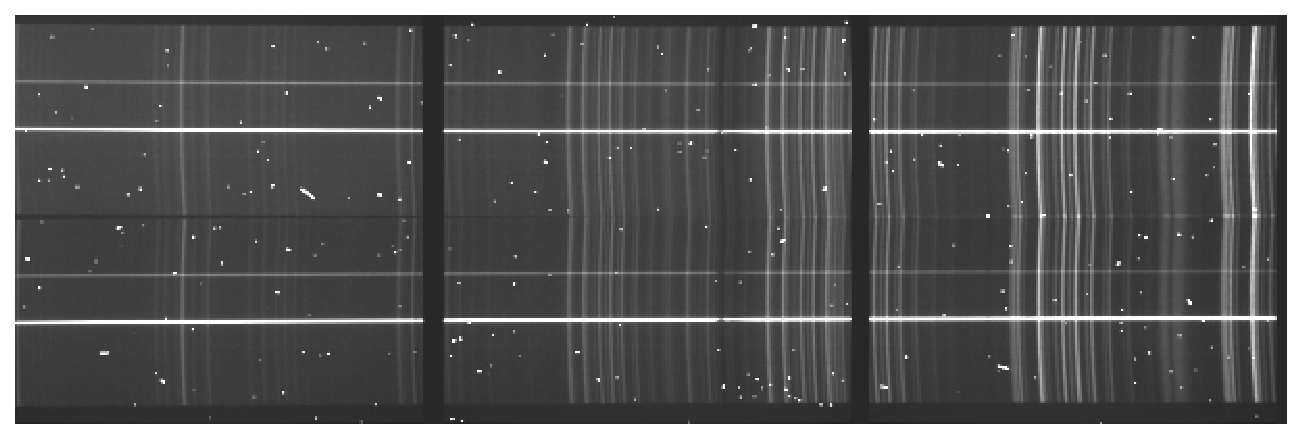
\includegraphics[width = 1.0\textwidth]{figures/3_pre_wav_cal.pdf}
    \caption{The science extension of a typical \polsalt \acs{FITS} file after basic \gls{CCD} reductions have been completed.}
    \label{fig:polsalt_pre_wav_cal}
\end{figure}


\subsection{Splitting the POLSALT pre-calibration files}

% Why necessary
%   Mention steps before and how they return (especially) the file structure.
As mentioned previously, the format of the \gls{FITS} file created by \polsalt after basic \gls{CCD} reductions and that expected by \iraf to be used for the wavelength calibrations are incompatible. A typical \gls{FITS} file created by the \polsalt basic \gls{CCD} reductions process contains a primary header along with the various image extensions, all of which include the trace for both polarimetry beams, as seen in Figure~\ref{fig:polsalt_pre_wav_cal}. \iraf deals best with a singular trace, and therefore a singular polarization beam, at a time.
\prgph

In an attempt to simplify the \iraf reduction procedure it was decided to split the polarization beams into their own files, as the parameters of \iraf tasks generally handle lists of files better than subregions of the same \gls{HDU}, and generally allowed for easier calibrations further down the \iraf wavelength calibration process.
\prgph

% What it does -> Primary focus
%   All processes run & description of each. Focus on why.
The \polsalt files with basic \gls{CCD} reductions applied, namely \gls{FITS} files with the prefix `mxgbp' (\S~\ref{subsec:polsalt}), are used as the starting point for the supplementary tool's \texttt{split} method. Running \texttt{split} finds all the \gls{FITS} files for wavelength calibration within the working directory, creates two empty \gls{HDU} structures for each sub-extension of the \gls{FITS} file, and appends all science and header data necessary for wavelength calibration to the relevant \gls{HDU} structure.
\prgph

% Focus on minimizing changes and optimizing size
As the intent was always to parse the wavelength function back into \polsalt it was decided to keep these temporary \gls{FITS} files as light as possible. This is especially necessary when considering the amount of frames that must be taken for a single spectropolarimetric observation, and then how that increases for long term studies.
\prgph

\begin{figure}[t]
    \centering
    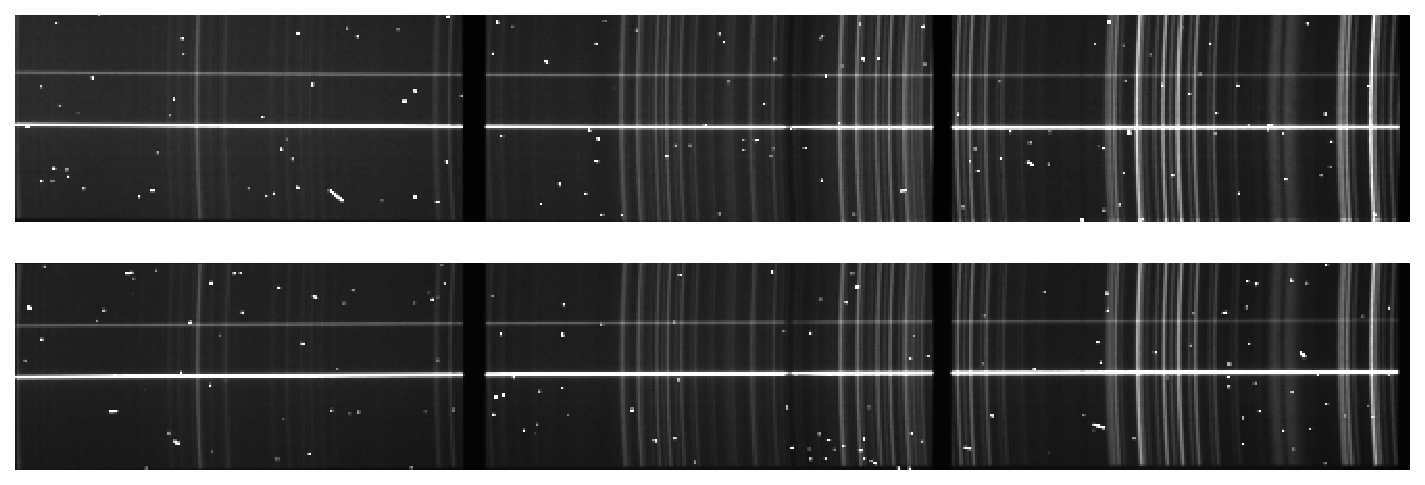
\includegraphics[width = 1.0\textwidth]{figures/3_OEsplit.pdf}
    \caption{The split $O$ and $E$ beams as handed to \iraf.}
    \label{fig:OE_split}
\end{figure}

% Any changes from how polsalt would do it
In an attempt to automate the scripting of the \iraf wavelength calibrations, row cropping was introduced into the \texttt{split} method to ignore the regions without a trace either side of the frame, and the creation of files listing the $O$ and $E$ beams. The row cropping was decided on as \iraf does not handle the empty rows well, specifically when it comes to the \texttt{reidentify} task. Otherwise, defaults, such as which row to split the beams along, were kept as close to the \polsalt pipeline as possible.


\subsection{IRAF wavelength calibration}\label{subsec:IRAF_wav_cal}

% What is IRAF and why necessary
\iraf is a collection of software designed specifically for the reduction and analysis of astronomical images and spectra. The software consists of many tasks which perform specific operations and which are grouped into relevant packages. As every researcher, university, and research group have their own preferred wavelength calibration procedures and often use specific parameters for the various \iraf tasks (e.g. the order and type of the polynomial used in \texttt{identify}, etc.) only a brief overview of the tasks used will be provided here.
\prgph

A useful \iraf task that will not be discussed but nevertheless deserves a mention is the \texttt{mkscript} task in the \texttt{system} package which allows a user to create and save a task along with the defined parameters as a file which can later be called as a script. It is instrumental as a scripting aid and is what allows \iraf its rapid recalibrations of the wavelength solutions.
\prgph

For the alternate wavelength calibrations, the relevant tasks, in order, are \texttt{identify} and \texttt{reidentify} located in the \texttt{noao.onedspec} package, and the \texttt{fitcoords} and optionally the \texttt{transform} tasks located under the \texttt{noao.twodspec.longslit} package. These tasks produce a two-dimensional wavelength solution and thus must all be run twice to create the different wavelength solutions for each of the two spectropolarimetric beams.


% What it does -> Primary focus
%   All processes run & description of each. Focus on why.
% https://astro.uni-bonn.de/~sysstw/lfa_html/iraf/noao.onedspec.identify.html#h_29
\paragraph{Identify}
The \texttt{identify} task is used to interactively determine a one-dimensional wavelength function across a chosen row of an arc exposure by identifying features in the spectrum with known wavelengths. \texttt{identify} gives the first approximation of the wavelength solution, which is saved to a local database, and is built on in subsequent tasks. It is thus imperative that the initial fit is done well to minimize errors further down the calibration process.
\prgph

The process of using \texttt{identify} consists of identifying known features spanning the entire wavelength range and then removing identified features which negatively impact the wavelength solution. A balance must be found between the number of identified features and parameters of the fit against the deviation of the fit from the known features. % RMS

% https://astro.uni-bonn.de/~sysstw/lfa_html/iraf/noao.onedspec.reidentify.html#h_29
\paragraph{Reidentify}
The \texttt{reidentify} task is used to run the \texttt{identify} task autonomously and repeatedly across the entirety of the arc exposure at a defined interval. \texttt{reidentify} uses the one-dimensional wavelength solution stored in the database created by the initial \texttt{identify} call and shifts the identified points to match their known spectral features. The task may fail based on a number of defined conditions, most common of which is the loss of features as the task moves further from the row at which the user ran \texttt{identify}.
\prgph

When running \texttt{reidentify} non-interactively, it is recommended to set the \texttt{verbose} parameter to `\texttt{yes}' as this will allow immediate confirmation whether the task quit early or not. Regardless of where the task ended, the newly defined wavelength solutions are appended to the local database.

% https://astro.uni-bonn.de/~sysstw/lfa_html/iraf/noao.twodspec.longslit.fitcoords.html
\paragraph{Fitcoords}
The \texttt{fitcoords} task is used to combine the collection of one-dimensional wavelength solutions in the local database to a two-dimensional surface function. This surface function is the final two-dimensional wavelength solution and is what is needed to convert the \iraf formatted wavelength calibrated \gls{FITS} files back into the \polsalt format.
\prgph

The process of using \texttt{fitcoords}, follows closely to that of \texttt{identify} and consists of examining the distribution of identified points and eliminating any points that \texttt{reidentify} may have misidentified. By eliminating outliers with bad residuals and modifying the two-dimensional surface function type and degree, the overall error of the fit decreases, matching more closely to what the `true' wavelength solution is.

% https://astro.uni-bonn.de/~sysstw/lfa_html/iraf/noao.twodspec.longslit.transform.html
\paragraph{Transform}
The \texttt{transform} task is an optional step in the \iraf wavelength calibration process but is good to perform since it is quick to run and easy to script. \texttt{transform} converts the ($pixel$, $pixel$) units stored in the exposure to ($wavelength$, $pixel$) units which allows for an immediate check of whether the wavelength solution was found correctly. Any error in the wavelength solution will be easily spotted in the transformed images and may range from minor, such as the arc exposure's arc lines or science exposure's sky lines not being straight across the columns of the frame, to more severe, such as the wavelength solution completely readjusting the frame to an incoherent mess.

\todo{Include poor and good transformed image examples?}


\subsection{Joining the wavelength calibrated files}

As mentioned previously, the format of the \gls{FITS} file created by \iraf after wavelength calibrations and that expected by \polsalt for the \texttt{spectral extraction} are incompatible. A typical \gls{FITS} file expected by the \polsalt \texttt{spectral extraction} contains a primary header along with the various image extensions, the most notable extension being the newly added wavelength extension. All images contained within the extensions have the trace for both polarimetry beams split, as seen in Figure~\ref{fig:polsalt_post_wav_cal} and the headers of each extension updated.
\prgph

All pieces necessary to recreate the \polsalt wavelength calibrated \gls{FITS} files exist once the \iraf procedure to generate the database entry for the two-dimensional wavelength solution is complete. The \texttt{join} method of the supplementary tools is used at this point and, once run, autonomously creates the desired files.
\prgph

Running \texttt{join} finds all the relevant \gls{FITS} and local database files necessary to run the \polsalt \texttt{spectral extraction}, creates an empty \gls{HDU} structure for each pair of matching spectropolarimetric beams, copies over the extensions and their respective image and header information, checks and corrects the trace splitting to best match that of \polsalt, appends a new extension and parses the database wavelength solutions into the \polsalt intensity-wavelength format, cleans the science extension for cosmic rays, and does some house-cleaning to align the finalized \gls{FITS} files to those created when using the `pure' \polsalt pipeline.
\prgph

% update headers
% copy data, double check shape change
The \gls{FITS} files created by the \texttt{join} method and \polsalt pipeline's \texttt{wavelength calibration} methods are almost identical. The only difference between the \gls{FITS} files is the shape of the images stored within them, reflected also through specifically the `NAXIS2' header keyword, since \texttt{split} introduces a cropping. It was deemed unnecessary to reintroduce the cropped region as it is promptly discarded in the following \polsalt \texttt{spectral extraction} process and raises no issues when left out. Otherwise, both the \texttt{join} method and \polsalt \texttt{wavelength calibration} update the headers to reflect the new shape of the data and data type, through header keywords `CTYPE3' and `BITPIX', respectively.
\prgph

% append new extensions
% How db converted to wav func
The wavelength extension is created entirely by \texttt{join} by appending a blank extension to the \gls{HDU} and filling the image pixels with their respective wavelength value. This is done entirely by \texttt{join} which parses the wavelength database file and creates a function which provides the corresponding wavelength when provided with a ($pixel$, $pixel$) position. This is used to fill the pixels of the wavelength extension with their respective wavelength, as seen in Figure~\ref{fig:pol_wav_ext}.

\begin{figure}[t]
    \centering
    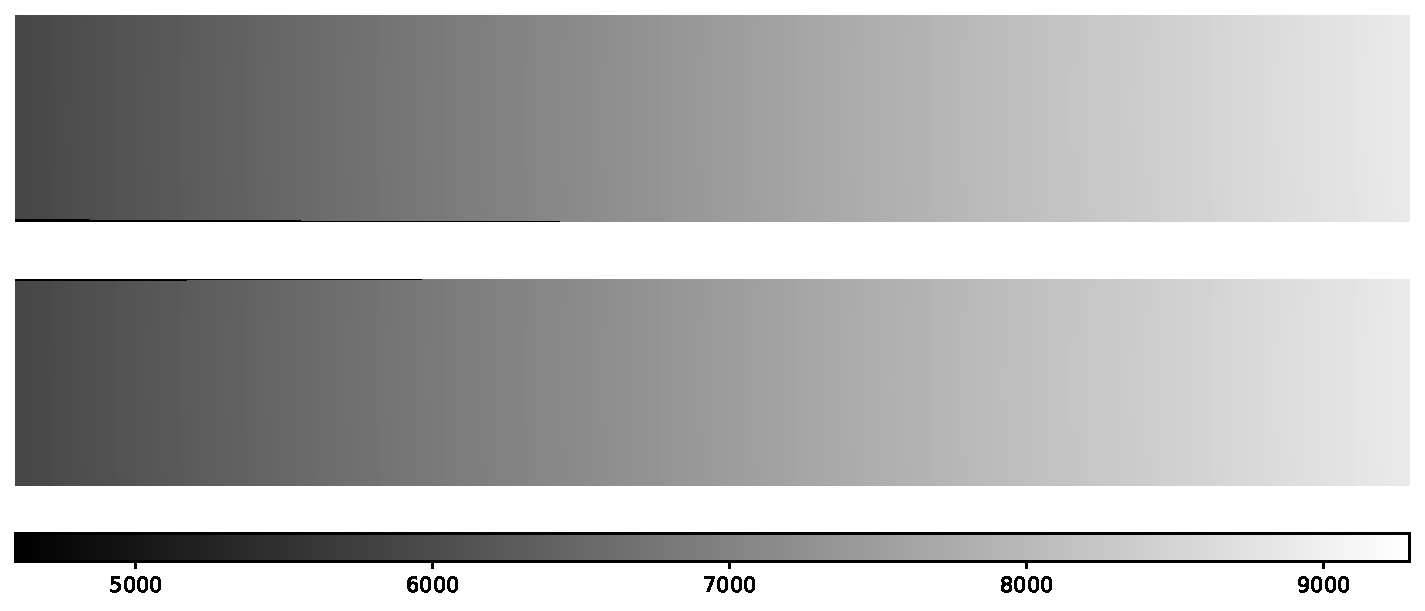
\includegraphics[width = 1.0\textwidth]{figures/3_pol_wav_ext.pdf}
    \caption{The wavelength extension of a \gls{FITS} file ready to be handed back to the \polsalt pipeline.}
    \label{fig:pol_wav_ext}
\end{figure}


% parse and save wavelength functions as image
% cosmic ray cleaning
% polsalt specific cropping (wav mask)
% mask wavelength using wollaston curve for polsalt `parsability'
% update BPM to reflect wavelength cropping

\todo{Return file structuring.}
\prgph

\todo{Focus on \textbf{why}. Parsing \iraf frames to be used by POLSALT and making sure the header and extensions reflect the changes}

\begin{figure}[t]
    \centering
    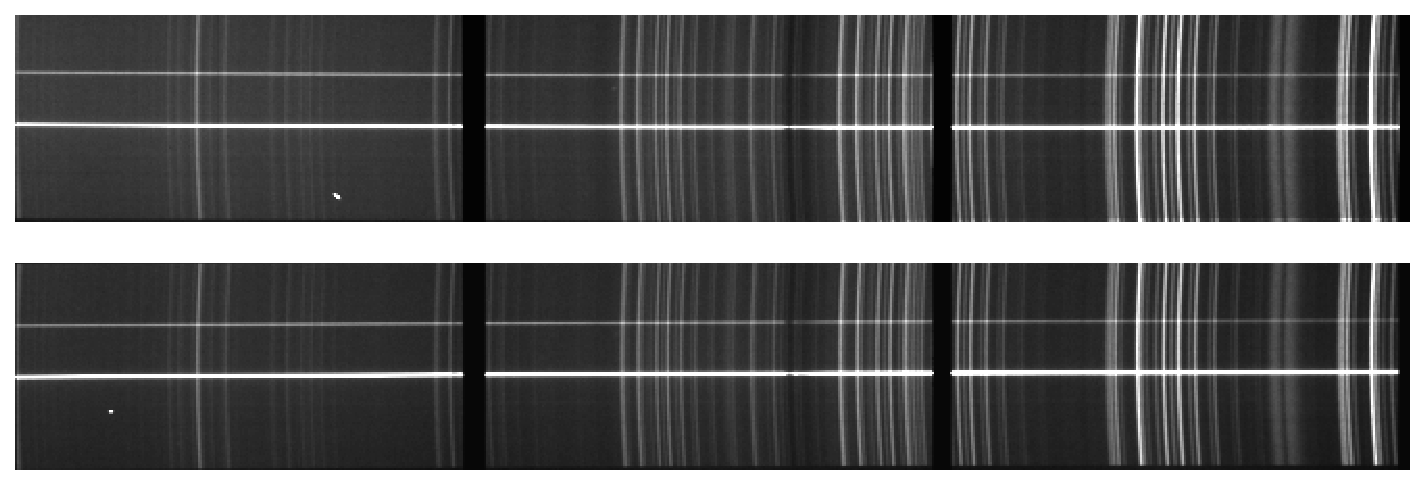
\includegraphics[width = 1.0\textwidth]{figures/3_post_wav_cal.pdf}
    \caption{The science extension of a \gls{FITS} file ready to be handed back to the \polsalt pipeline.}
    \label{fig:polsalt_post_wav_cal}
\end{figure}


\section{Additional Tools}\label{sec:add_tools}

Along with the ability to perform wavelength calibrations in \iraf, it was deemed necessary to create tools to allow for the comparison of the $O$ and $E$ beams.

\todo{fill out}

\subsection{Cross correlation}

\todo{Why a cross correlation necessary and how it works}


\subsection{Skyline comparisons}

\todo{REMOVE? Not truly implemented... Again, why a skyline comparison necessary and how it works. Also, how the frame is transformed (\iraf bypassed) and that the flux is not conserved so only for checking and not for science use.}


\section{General Reduction Procedure}\label{sec:red_proc}

\begin{figure}[t]
    \centering
    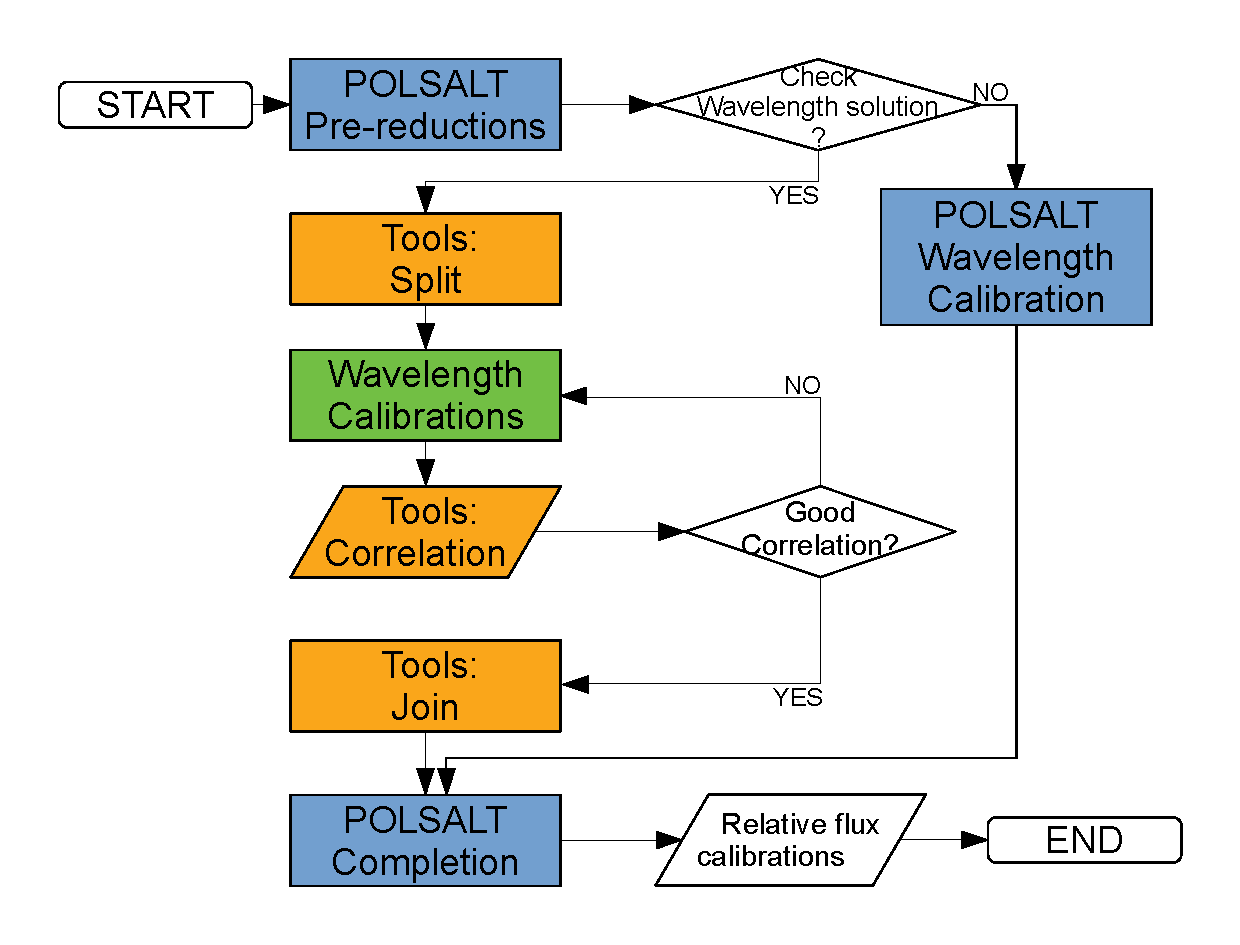
\includegraphics[width = 0.7\textwidth]{figures/3_new_workflow.pdf}
    \caption{A general workflow for data reductions using a combination of \polsalt, \iraf, and the developed supplementary tools.}
    \label{fig:new_workflow}
\end{figure}

\todo{General reduction procedure from raw data to finalized results
    \begin{itemize}
        \item This includes \polsalt pre-reductions, splitting, \iraf wavelength calibrations, checking, joining, and \polsalt finalization. (Include Relative flux calibrations for `shape correcting' spectrum??)
        \item mention help docs of sup. tools.
    \end{itemize}
}